\section{User Interface Representation (Of  Respective Project)}
No matter how new technologies change our lifestyle, people will always shop. Developing and designing mobile apps for ecommerce businesses has its own tricks. And online shopping follows adheres to the same principles as offline shopping. If customers don’t like what they see, they won’t buy. That’s why intuitive interfaces and catchy designs are invaluable for any ecommerce app.

We analyse user behaviour and design apps that cater to our users needs. For this article, we asked our design department to share their tips and tricks for designing an ideal ecommerce app.

Ecommerce apps contain three essential components: a catalogue (list of goods), search and filter options, and a shopping cart (or checkout).

\subsection{Snapshots of system}


\begin{figure}[ht]
\centering
\includegraphics[scale=0.30]{images/1.png}
\caption{Login Screen}

Here the back end connectivity used if fire base. When user login to the account the new account is made in fire base. In order to login one has to confirm the email in his account. Then he/she can login in application.

\end{figure}

\newpage

\begin{figure}[ht]
\centering
\includegraphics[scale=0.30]{images/2.png}
\caption{Register Screen}

If the user doe snot have previous account details or he/she is a new user, he has to register first to login.

\end{figure}

\newpage

\begin{figure}[ht]
\centering
\includegraphics[scale=0.30]{images/g1.png}
\caption{Items Cart}

This photo represents the items which can be purchased from the application. this contain a custom list view with an adapter.

\end{figure}

\newpage

\begin{figure}[ht]
\centering
\includegraphics[scale=0.30]{images/4.png}
\caption{Navigation Drawer}

This photo shows the navigation drawer. The library used in the development is of mike penz which completely solves our purpose to show the attached links of the project.

\end{figure}

\newpage

\begin{figure}[ht]
\centering
\includegraphics[scale=0.30]{images/g2.png}
\caption{Shopping Cart}
\end{figure}

\newpage

\begin{figure}[ht]
\centering
\includegraphics[scale=0.30]{images/g3.png}
\caption{Payment Gateway (PayuMoney)}

Payumoney is an affordable on line payment gateway provider in India. It enable small business to integrate on line payment gateway services without any set-up cost.

\end{figure}



\newpage

\begin{figure}[ht]
\centering
\includegraphics[scale=0.30]{images/10.png}
\caption{Payment Gateway Login}

In order to complete the payment successfully one has to fill his email id. This email id is taken to send the status of the payment to the email.
\end{figure}

\newpage

\begin{figure}[ht]
\centering
\includegraphics[scale=0.30]{images/11.png}
\caption{Register to gateway}

You can also make account in the payment gateway for easy and fast transaction processing. You can also save your card which make payment more faster.
\end{figure}

\newpage

\begin{figure}[ht]
\centering
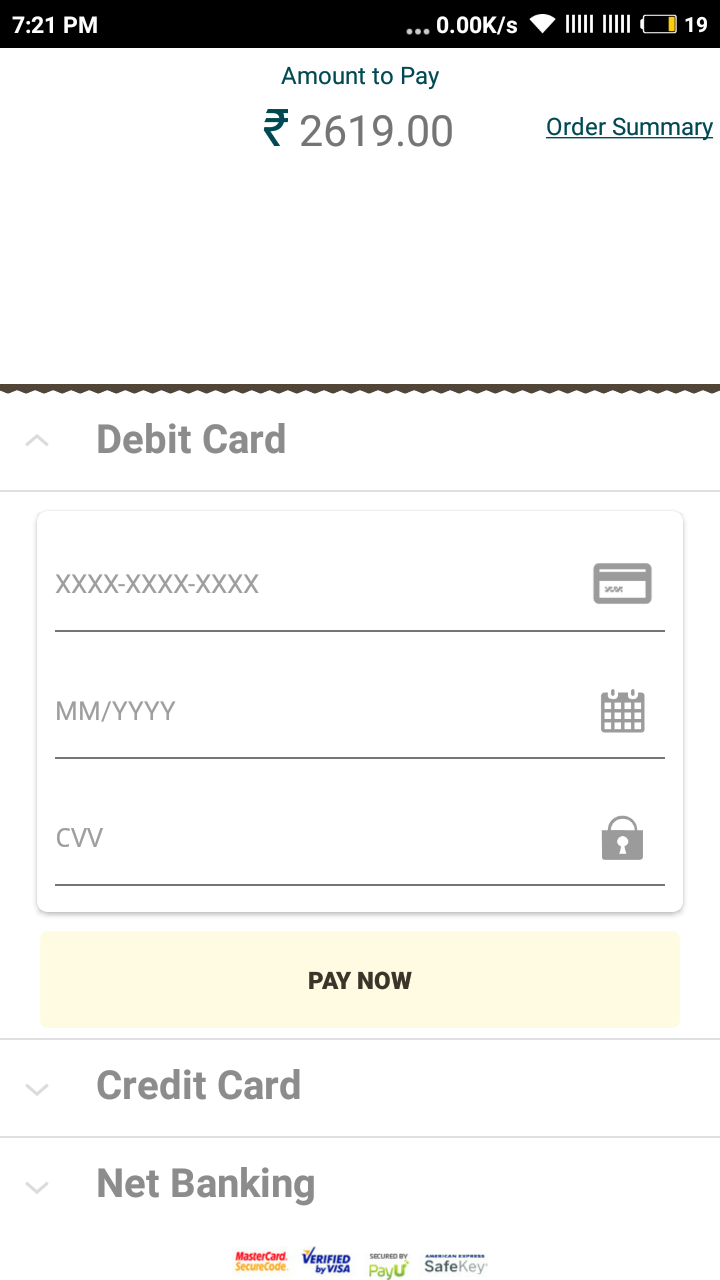
\includegraphics[scale=0.30]{images/cardcheckout.png}
\caption{Payment}

We can use debit card, credit card, net banking method for payment of the products purchased.

\end{figure}

\newpage

\begin{figure}[ht]
\centering
\includegraphics[scale=0.30]{images/12.png}
\caption{About us}
\end{figure}

\newpage

\begin{figure}[ht]
\centering
\includegraphics[scale=0.30]{images/13.png}
\caption{Enquiry Bot}
This bot is developed in Api.ai (Dialogflow). It give users new ways to interact with your product by building engaging voice and text-based conversational interfaces powered by AI. Connect with users on the Google Assistant, Amazon Alexa, Facebook Messenger, and other popular platforms and devices. 
\end{figure}

\newpage

\begin{figure}[ht]
\centering
\includegraphics[scale=0.30]{images/14.png}
\caption{Share Application}

We can share our application with approximately all the platforms easily.

\end{figure}

\newpage

\begin{figure}[ht]
\centering
\includegraphics[scale=0.30]{images/15.png}
\caption{Feedback}

We are ready to take the feedback from our user for the app improvement and UI/UX interaction for growth.
\end{figure}

\section{Back Ends Representation (Database to be used)}
\subsection{Firebase Realtime Database}
Store and sync data with our NoSQL cloud database. Data is synced across all clients in realtime, and remains available when your app goes offline.

The Firebase Realtime Database is a cloud-hosted database. Data is stored as JSON and synchronized in realtime to every connected client. When you build cross-platform apps with our iOS, Android, and JavaScript SDKs, all of your clients share one Realtime Database instance and automatically receive updates with the newest data.
\subsection{How does it work?}
The Firebase Realtime Database lets you build rich, collaborative applications by allowing secure access to the database directly from client-side code. Data is persisted locally, and even while offline, realtime events continue to fire, giving the end user a responsive experience. When the device regains connection, the Realtime Database synchronizes the local data changes with the remote updates that occurred while the client was offline, merging any conflicts automatically.

The Realtime Database provides a flexible, expression-based rules language, called Firebase Realtime Database Security Rules, to define how your data should be structured and when data can be read from or written to. When integrated with Firebase Authentication, developers can define who has access to what data, and how they can access it.

The Realtime Database is a NoSQL database and as such has different optimizations and functionality compared to a relational database. The Realtime Database API is designed to only allow operations that can be executed quickly. This enables you to build a great realtime experience that can serve millions of users without compromising on responsiveness. Because of this, it is important to think about how users need to access your data and then structure it accordingly.



\subsection{Snapshots of Database}

\newpage

\begin{figure}[ht]
\centering
\includegraphics[scale=0.50]{images/firbase14.png}
\caption{Confirmation Email in Fire base}
\end{figure}

